\subsection{Variables de entrada}
Son las fuentes que suministran energía al sistema. Habrá un total de tres:
\begin{itemize}
	\item \textbf{Energía fotovoltaica (EF)}\\ Energía procedente de las placas solares. Su valor viene determinado por varios factores, como son el número de módulos fotovoltaicos instalados y la máxima potencia que puede generar en cada momento, \gls{CMP}. Hace referencia a la potencia de salida, en watios que produce un panel fotovoltaico en condiciones de máxima iluminación solar, con una radiación de aproximadamente 1 kW/m2. Será dependiente de la situación meteorológica del momento. Como se puede observar, tendrá un valor máximo de obtención, que representa la cantidad de energía máxima que podemos obtener de los módulos fotovoltaicos en ese momento.
	\item \textbf{Energía de red (ER)}\\ Energía procedente de la compañía eléctrica como cliente particular. Al contrario que en el caso anterior, no existe un límite superior a la hora de obtener energía de esta fuente.
	\item \textbf{Energía almacenada en batería (EB)}\\ Energía obtenida de la batería de almacenaje. Al igual que la energía fotovoltaica tiene un límite superior y viene determinado por la cantidad de carga de la misma y la profundidad de descarga que se le puede realizar sin perjudicar su ciclo de vida y que debe ser de un 50\% como máximo.
\end{itemize}
\subsection{Adquisición de valores para las variables}
Como se ha mencionado, la energía fotovoltaica en una hora t será dependiente de la situación meteorológica en ese instante, algo evidente. Para contar con información meteorológica existen conjuntos de herramientas o servicios que ponen dicha información a disposición del desarrollador, como por ejemplo una API. Una \gls{API} es un conjunto de reglas o especificaciones que permite a las aplicaciones proporcionar servicios a otras o comunicarse. En este \gls{TFG} se emplea la \gls{API} oficial de AEMET \cite{Aemet}. Para su uso, se ha debido solicitar un \textbf{API key} ya que es una \gls{API} cerrada, esto es, su uso está restringido a un conjunto limitado de clientes. Para realizar una petición a la misma, debe incluirse el \textit{API key} mencionado anteriormente en la url solicitada, así como una serie de parámetros como el código del municipio que se desea consultar. Para obtener y procesar la información recibida por la \gls{API} se ha creado el módulo \textit{api\_aemet}, que contiene dos funciones para la obtención de información, una que se encarga de obtener la información referente al día en curso y otra que se encarga de obtener la información cuando la simulación se desea realizar de un día concreto. El motivo de diferenciarlas es que la \gls{API} no realiza una respuesta con predicciones por horas de un día distinto al actual, devolviendo en su defecto un texto en lenguaje natural con un resumen de lo ocurrido meteorológicamente dicho día para estos casos. Dichas funciones se explican a continuación.
\begin{itemize}
\item \textit{\textbf{get\_weather\_today}} (Listado~\ref{lst:aemet1}). Esta función realiza una petición a la \gls{API} mediante la librería \textit{requests}~\cite{Kenn11}, y en caso de obtener un código de éxito (código de estado http 200), procesa la respuesta recibida. Dicha respuesta es fácilmente es un conjunto de parámetros clave-valor. Se procesa en la función \textbf{create\_weather\_buffer} y devuelve una lista con los 24 estados meteorológicos, correspondientes a las 24 horas de la simulación, del tipo ["Despejado", "Poco Nuboso", "Despejado", ..., "Despejado"].
\begin{lstlisting}[language=Python,float=ht,caption={Función para obtener los valores meteorológicos del día en curso},label={lst:aemet1}]
def get_weather_today(city):
    weather_buffer = []
    url = const.AEMET_URL_NOW.replace('$CITY', city)
    response = requests.get(url)
    data = response.json()

    if data['estado'] == 200:
        url = data['datos']
        response = requests.get(url)
        data = response.json()[0]
        weather_buffer = create_weather_buffer(data)
        return weather_buffer
    return None
\end{lstlisting}

\item \textit{\textbf{get\_weather\_archive}} (Listado~\ref{lst:aemet2}). Esta función realiza la petición a la \gls{API} de manera similar a la anterior, salvo que debe incluir en la url el parámetro específico de la fecha que se desea consultar. En este caso la respuesta no es directamente procesable pues no se trata de parámetros clave-valor. En su lugar se ha de procesar un texto en lenguaje natural (obsérvese en el Listado~\ref{lst:aemet1} como la respuesta es convertida a \textit{json} y en este caso es convertida a \textit{text}). Para su resolución, se ha implementado la función \textit{process\_weather\_archive} que realiza una \textbf{búsqueda de ocurrencias} de estados meteorológicos conocidos en el texto en lenguaje natural, obteniendo así información acerca del estado meterológico que se produjo ese día. Se forma el buffer con los estados meteorológicos encontrados en el texto y se devuelve una lista similar a la del caso anterior. En el Listado~\ref{lst:APIresponse2} se muestra un ejemplo del tipo de respuesta obtenida. En este caso se encontraría una ocurrencia de un estado meteorológico ('despejados'), por lo tanto se formaría el buffer del estado del cielo con 'Despejado'.
\begin{lstlisting}[language=Python,float=ht,caption={Función para obtener los valores meteorológicos de un día concreto},label={lst:aemet2}]
def get_weather_archive(date, city):
    weather_buffer = []
    province = city[:2]
    url = const.AEMET_URL_DATE.replace('$PROVINCE', province).replace('$DATE', date)

    response = requests.get(url)
    data = response.json()

    if data['estado'] == 200:
        url = data['datos']
        response = requests.get(url)
        raw_info = response.text
        weather_buffer = process_weather_archive(raw_info)
        return weather_buffer
    else:
        return None
\end{lstlisting}
\begin{lstlisting}[numbers=none,float=ht,caption={Ejemplo de respuesta de la API-AEMET para un día diferente al actual},label={lst:APIresponse2}]
AGENCIA ESTATAL DE METEOROLOGÍA

PREDICCIÓN PARA LA PROVINCIA DE TOLEDO
DÍA 12 DE FEBRERO DE 2019 A LAS 14:01 HORA OFICIAL
PREDICCIÓN VALIDA PARA EL MARTES 12


TOLEDO

Cielos despejados. Temperaturas mínimas en descenso. Temperaturas
máximas con pocos cambios predominando los aumentos en la Mancha.
Vientos flojos del este y nordeste tendiendo a flojos variables.
\end{lstlisting}
\end{itemize}

Las variables de entrada pueden tener simultaneamente valores distintos de 0, es decir, se puede obtener un tanto por ciento de la energía requerida de cada una de ellas. La selección de una u otra vendrá determinado por el precio en ese momento de cada una, ya que lo que se busca es minimizar el gasto producido. A continuación se muestran los cálculos que permiten determinar los precios asociados a las variables de entrada en una hora t: \\

	El precio de la energía fotovoltaica se calcula a partir de la inversión realizada en la instalación de los módulos fotovoltaicos y la cantidad de años en los que se desea amortizar dicha inversión. Así, el precio en €/Kw de EF se toma a partir de la Ecuación~\ref{eq:costoEF}.
	\begin{equation}
          \label{eq:costoEF}
	Costo_{EF} = \frac{coste_{anual}}{promedio^{kw}_{anual}} \textup{\euro}/kw
	\end{equation}
	Siendo el coste anual la cantidad invertida entre el número de años(n) en amortizarla, como se puede observar en la Ecuación~\ref{eq:inversionEF}
	\begin{equation}
          \label{eq:inversionEF}
	Coste_{anual} = \frac{inversion}{n} \textup{\euro}
	\end{equation}


	El precio de la energía de red se obtiene haciendo uso de la \gls{API} oficial de \gls{REE} (e-sios) \cite{Ree}. Se ha debido solicitar un \textit{Token} de acceso que se utiliza en las llamadas a la misma al tratarse de una \gls{API} cerrada, análogamente al caso de la \gls{API} de AEMET. Para trabajar con esta \gls{API} se ha creado el módulo \textit{api\_esios}, que contiene la función \textit{get\_incoming\_prices}, la cuál se muestra en el Listado~\ref{lst:esios}.

	\begin{lstlisting}[language=Python,float=ht,caption={Función para obtener el precio del mercado eléctrico},label={lst:esios}]
	def get_incoming_prices(indicator, start, end):
	   url = const.ESIOS_URL.replace('$INDICATOR', indicator)
	   url = url.replace('$START_DATE', dt.datetime.strftime(start, '%Y/%m/%d'))
	   url = url.replace('$END_DATE', dt.datetime.strftime(end, '%Y/%m/%d'))

	   response = requests.get(url, headers=HEADERS)
	   if response.status_code == 200:
	      data = response.json()
	      price_buffer = create_price_buffer(data, start)
	      return price_buffer
	   return None
	\end{lstlisting}

	Esta función es llamada desde el proyecto con el indicador, que se corresponde con el precio que se desea consultar (en este caso \gls{PVPC}). Su código numérico es obtenido de las constantes del proyecto, al igual que la url necesaria para la petición (ESIOS\_URL), que se forma con los parámetros adecuados y así se realiza la petición \textit{get} haciendo uso de la librería \textit{requests}~\cite{Kenn11}.\\En este caso el \textit{\gls{API} key} no se concatena en la url, si no que debe incluirse en la cabecera de la petición en un campo específico, ya que se trata de una autenticación por token. Si la petición ha sido exitosa (código de respuesta http 200), la función retornará un \textit{buffer} de tamaño 24, que se corresponde con los valores del \gls{PVPC} en las 24 horas de un día. Para ello llama a \textit{create\_price\_buffer}, que se encargará de generar la lista con los 24 valores del precio. De esta manera se consigue el precio por Kw de la energía de red.

	Por último, el precio de la energía para las baterías se puede calcular de un modo muy parecido al de la energía fotovoltaica. Hace referencia al coste que supone extraer energía almacenada en la batería y está relacionado con la inversión realizada en su adquisición(Ecuación~\ref{eq:costoEB}).
	\begin{equation}
          \label{eq:costoEB}
	Costo_{EB} = \frac{coste_{anual}}{capacidad_{bat}\cdot182,5} \textup{\euro}/kw
	\end{equation}
	Habiendo obtenido previamente el coste anual de forma similar a la Ecuación~\ref{eq:inversionEF}. La constante 182,5 hace referencia al número de días del año (365) multiplicado por 0,5, debido a que no se va a realizar una profundidad de descarga mayor al 50\% de la capacidad total de la batería. El valor obtenido es el precio que supone extraer 1 Kw de la batería.
\subsection{Variables de salida}
Representan las fuentes de consumo de energía en el sistema. Habrá un total de cuatro:
\begin{itemize}
\item \textbf{Consumo del hogar (C)}\\Demanda energética del hogar en cuestión, cuantía que debe ser satisfecha siempre, ya que es la energía que necesita el hogar para su uso cotidiano. En este \gls{TFG} se ha decidido trabajar con clientes de la empresa eléctrica Endesa S.A., pues el hogar del alumno es su cliente lo que permitirá trabajar con información real. Además cuenta con un área privada de cliente que permite acceder a datos analíticos del hogar (Figura~\ref{fig:endesa}) y permite descargar ficheros en formato de texto con el consumo por horas de un día determinado, justo lo que se necesita para asignar valores a esta variable. Para adaptar la información del fichero al valor de la variable se ha creado la función \textit{read\_from\_file(filename)} del módulo \textit{client\_consumption} que devuelve una lista con los consumos de las 24 horas de un día en KW.
  \begin{figure}[H]
    \centering
    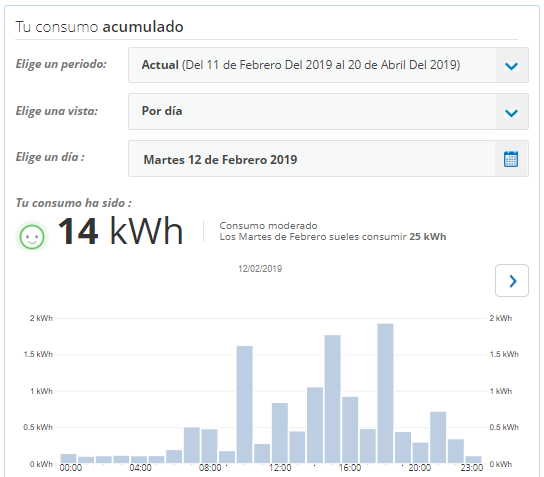
\includegraphics[width=10cm]{figs/Endesa.PNG}
    \caption{Panel de control del área de cliente de Endesa}
    \label{fig:endesa}
  \end{figure}
\item \textbf{Consumo interno del sistema ($ C_{int} $)}\\El sistema propuesto tiene un consumo constante de funcionamiento, cuyo valor se ha estimado en aproximadamente 2 Kw al día, alrededor de unos 0,088 watios por hora. Aquí se considera el consumo para el funcionamiento de las placas fotovoltaicas y para la realización de carga y descarga de la batería.
	\item \textbf{Carga de batería (CB)}\\Cantidad de energía que se almacena en la batería para su posterior uso. Esta variable cobra sentido en el caso de un abaratamiento de alguna fuente de generación de energía, así se almacena para cuando el precio sea mayor.
	\item \textbf{Vertido al mercado eléctrico (CR)}\\Cantidad de energía que se vende al mercado eléctrico. Como particular, se puede disponer de una instalación fotovoltaica y verter energía a la red eléctrica, aunque es una práctica sujeta a numerosas trabas legales y dificultades en las que no se entrará en el desarrollo de este \gls{TFG}. Esta energía se vertería al intramercado de red conocido como el mercado SPOT, aquel donde los activos que se compran o venden se entregan al precio de mercado del instante de la compra/venta.
\end{itemize}

Como se puede observar, el vertido al mercado eléctrico tiene un beneficio económico que ha de tenerse en cuenta. Existe una retribución por Kw vertido a la red dependiente del momento del día, ya que como se ha comentado antes, el valor de compra/venta del mercado SPOT varía. Para la obtención de estos valores se vuelve a hacer uso de la ya mencionada \gls{API} e-sios, proporcionando a la función \textit{get\_incoming\_prices} el indicador del precio SPOT, presente en el fichero de constantes del proyecto. Análogo a la obtención del \gls{PVPC}, se retorna un conjunto con los 24 valores requeridos del precio SPOT correspondientes a las 24 horas a simular.\\

Aunque a priori parezca que el hecho de cargar las baterías no tiene una compensación económica, esto no es del todo correcto. Existe un beneficio económico, aunque no directo, con esta práctica. Puede ser explicado como la cantidad ahorrada por almacenar esa energía y no consumirla, ya que se ha pagado por ella. Este valor puede verse como el mínimo de los precios de las fuentes de generación de energía en el momento de la carga. Veamos un breve ejemplo: En la hora t se ha obtenido la energía necesaria de dos fuentes: Por un lado energía fotovoltaica a un precio de 0,11 € el Kwh. Por otro lado, energía de la compañía eléctrica contratada a un precio de 0,14 € el Kwh. El beneficio económico indirecto por cargar un Kw de energía en batería en esta hora t será de 0,11 €, que es el precio más barato de las fuentes utilizadas.

\subsection{Variables de control}
Existe otro conjunto de variables conocido como variables de control. Aunque se denotan como variables, en un caso concreto de optimización son constantes, ya que sus valores están predefinidos para esa simulación del modelo. Una simulación es un caso concreto de optimización del sistema en un hogar y día determinados. El conjunto de variables de control está formado por:
\begin{itemize}
	\item \textbf{Fecha de inicio}\\ Valor que hace referencia al inicio de la simulación. Este valor es representado mediante el módulo datetime de Python. Datetime~\cite{Dtpy} es un módulo de la librería estándar de Python que permite manipular y trabajar con fechas. Este valor será un día y una hora de ese día.
	\item \textbf{Fecha de fin}\\ Corresponde al fin de la simulación. Siempre será 24 horas a partir de la fecha de inicio. Al igual que el anterior, se representa haciendo uso de datetime.
	\item \textbf{Número de módulos fotovoltaicos}\\ El número de módulos fotovoltaicos juega un papel fundamental. A mayor número de módulos, se producirá mas energía, pero mayor deberá ser la inversión para adquirirlos.
	\item \textbf{Precio de un módulo fotovoltaico}\\ En este trabajo el tipo de módulo fotovoltaico será el que suele usar en domicilios particulares, con una potencia nominal en condiciones ideales de 50 watios. Este módulo tiene un precio por unidad de 40 €.
	\item \textbf{Años en amortizar la inversión de los módulos fotovoltaicos}\\ Número de años en los que se desea amortizar la inversión realizada en la adquisición de los módulos fotovoltaicos mediante su uso. Como se ha comentado anteriormente, no es algo trivial ya que determinará en gran medida el precio de extracción de energía fotovoltaica.
	\item \textbf{Precio de la batería}\\ En este trabajo el tipo de batería es una batería estacionaria compuesta por plomo abierto y gel. Este tipo de batería esta compuesta por dos vasos de 2V cada uno, que disponen de un amplio rango de autonomía y una vida útil bastante larga, alrededor de unos 20 años. Están aconsejadas en instalaciones con un consumo medio (microondas, horno, lavadora, aire acondicionado, etc). Como su tensión es de 2V, se deben instalar un total de 6 vasos en serie, al estar la instalación solar a 12V. Su precio es elevado debido a la gran capacidad, siendo éste 3900 €.
	\item \textbf{Capacidad de la batería}\\ El tipo de batería usado, es decir, batería estacionaria de 6 vasos, tiene una capacidad aproximada de 21 Kw. La profundidad de descarga de este tipo de batería es aproximadamente del 50\%, esto es, como se comento durante la explicación de las variables de entrada y salida, el tanto por ciento que se puede descargar dicha batería sin resultar perjudicial para su salud y por lo tanto afectar a su ciclo de vida útil.
	\item \textbf{Nivel de carga inicial de la batería}\\ Variable de control que define el estado de carga inicial de la batería a la hora de realizar la simulación de la optimización.
	\item \textbf{Años en amortizar la inversión de la batería}\\ Como ocurre en el caso de la inversión fotovoltaica, se debe determinar el número de años en los que se desea realizar la amortización de la inversión por adquirir la batería. Al tratarse de un precio mucho más elevado debe ser mayor al del caso anterior, ya que si no se dispararía el precio de descargar las baterías y dejaría de ser una entrada a tener en cuenta al no resultar rentable.
\end{itemize}
Con esto quedan identificadas cada una de las variables que entran en juego en el modelo, así como su medio de adquisición.
